\documentclass[UTF8]{ctexart}
\usepackage{../Zhihu}
\title{数字电路学习笔记(九):初识锁存器}
\begin{document}
\maketitle
所有的组合逻辑电路都只能实现计算功能——但计算机(以及大多数控制器)不能只会计算,还要能够存储数据。思考,如何用逻辑门实现存储数据的功能?

\section*{一、RS锁存器}
我们将能够存储一个状态的电路叫做锁存器。设想一个电路,初始输入为0,输出为0;然后输入为1,输出变为1(状态发生了变化)。对于迄今为止所有的电路,我们都能保证当输入回到0时,输出也会同时归0;但这个电路不同,它保持在了1,也就是状态没有发生变化,而是被存储了下来。此时,这种电路便可以被叫做锁存器。

为了让电路拥有自己的“状态”,必须要有某种“反馈”机制,将输出输入形成一个闭环。所以,锁存器的原型如下图:(它是如何设计出来的不重要;但接下来的所有元件都以它为基础)

\begin{figure}
    \begin{circuitikz}[scale=0.7, transform shape]
        \draw (2,2) node[not port] (not1) {1};
        \draw (2,0) node[not port] (not2) {2};
        \draw[green] (not1.out) -- ++(1,0) node[right, scale={1/0.7},black] {$Q$};
        \draw (not2.out) -- ++(1,0) node[right, scale={1/0.7}] {$Q'$};
        \draw (not1.in) -- ++(-0.3,0);
        \draw[green] (not2.in) -- ++(-0.3,0);
        \draw[green] (not1.out)++(0.3,0) to[short,*-,color=green] ++(0,-0.7) -- ([shift={(-0.3cm,0.7cm)}]not2.in) -- ++(0,-0.7);
        \draw (not2.out)++(0.3,0) to[short,*-] ++(0,0.7) -- ([shift={(-0.3cm,-0.7cm)}]not1.in) -- ++(0,0.7);

        \draw (7,2) node[not port] (not1) {1};
        \draw (7,0) node[not port] (not2) {2};
        \draw (not1.out) -- ++(1,0) node[right, scale={1/0.7}] {$Q$};
        \draw[green] (not2.out) -- ++(1,0) node[right, scale={1/0.7},black] {$Q'$};
        \draw[green] (not1.in) -- ++(-0.3,0);
        \draw (not2.in) -- ++(-0.3,0);
        \draw (not1.out)++(0.3,0) to[short,*-] ++(0,-0.7) -- ([shift={(-0.3cm,0.7cm)}]not2.in) -- ++(0,-0.7);
        \draw[green] (not2.out)++(0.3,0) to[short,*-,color=green] ++(0,0.7) -- ([shift={(-0.3cm,-0.7cm)}]not1.in) -- ++(0,0.7);
    \end{circuitikz}
\end{figure}

它有两种状态,可以看到,两种状态都是稳定的,第一种输出$Q=1,\,Q'=0$;第二种则是$Q=0,\,Q'=1$。可以顺着线路,看看循环是如何构成的。我们把这两种状态分别用$Q$表示,即$Q=0$状态和$Q=1$状态。对于所有的锁存器,都有$Q$和$Q'$两个输出,且它们必定相反。

但是,这种电路没有输入,一旦回路构成,它的输出就确定下来了。但我们在最开头所设想的锁存器是能根据输入改变自己的状态的。为了给输入留出空间,我们要把非门换成与非门或者或非门。(这也是一步拍脑袋的改进。锁存器的设计中,很少有能明确讲出所以然的操作,but it works, and that's all that matters.)

\begin{figure}
    \begin{circuitikz}[scale=0.7, transform shape]
        \draw (2,2) node[nor port] (not1) {1};
        \draw (2,0) node[nor port] (not2) {2};
        \draw (not1.out) -- ++(1,0) node[right, scale={1/0.7}] {$Q$};
        \draw[green] (not2.out) -- ++(1,0) node[right, scale={1/0.7},black] {$Q'$};
        \draw (not2.in 1) -- ++(-0.3,0);
        \draw[green] (not1.in 2) -- ++(-0.3,0);
        \draw (not1.out)++(0.3,0) to[short,*-] ++(0,-0.7) -- ([shift={(-0.3cm,0.5cm)}]not2.in 1) -- ++(0,-0.5);
        \draw[green] (not2.out)++(0.3,0) to[short,*-,color=green] ++(0,0.7) -- ([shift={(-0.3cm,-0.5cm)}]not1.in 2) -- ++(0,0.5);
        \draw (not1.in 1) -- ++(-1,0) node[left,scale={1/0.7}] {$R$};
        \draw (not2.in 2) -- ++(-1,0) node[left,scale={1/0.7}] {$S$};

        \draw (8,2) node[nand port] (not1) {1};
        \draw (8,0) node[nand port] (not2) {2};
        \draw (not1.out) -- ++(1,0) node[right, scale={1/0.7}] {$Q$};
        \draw[green] (not2.out) -- ++(1,0) node[right, scale={1/0.7},black] {$Q'$};
        \draw (not2.in 1) -- ++(-0.3,0);
        \draw[green] (not1.in 2) -- ++(-0.3,0);
        \draw (not1.out)++(0.3,0) to[short,*-] ++(0,-0.7) -- ([shift={(-0.3cm,0.5cm)}]not2.in 1) -- ++(0,-0.5);
        \draw[green] (not2.out)++(0.3,0) to[short,*-,color=green] ++(0,0.7) -- ([shift={(-0.3cm,-0.5cm)}]not1.in 2) -- ++(0,0.5);
        \draw[green] (not1.in 1) -- ++(-1,0) node[left,scale={1/0.7},black] {$S$};
        \draw[green] (not2.in 2) -- ++(-1,0) node[left,scale={1/0.7},black] {$R$};
    \end{circuitikz}
\end{figure}

我们逐个分析,看它们的输出是如何变化的。

1、或非门锁存器
首先,初始状态是$Q=R=0$,此时电路处于双稳态——$Q=0$和$Q=1$都是稳定状态;接下来,分别令$S=1$和$R=1$:

\begin{figure}
    \begin{circuitikz}[scale=0.7, transform shape]
        \draw (2,2) node[nor port] (not1) {1};
        \draw (2,0) node[nor port] (not2) {2};
        \draw (not1.out) -- ++(1,0) node[right, scale={1/0.7}] {$Q$};
        \draw[green] (not2.out) -- ++(1,0) node[right, scale={1/0.7},black] {$Q'$};
        \draw (not2.in 1) -- ++(-0.3,0);
        \draw[green] (not1.in 2) -- ++(-0.3,0);
        \draw (not1.out)++(0.3,0) to[short,*-] ++(0,-0.7) -- ([shift={(-0.3cm,0.5cm)}]not2.in 1) -- ++(0,-0.5);
        \draw[green] (not2.out)++(0.3,0) to[short,*-,color=green] ++(0,0.7) -- ([shift={(-0.3cm,-0.5cm)}]not1.in 2) -- ++(0,0.5);
        \draw (not1.in 1) -- ++(-1,0) node[left,scale={1/0.7}] {$R$};
        \draw (not2.in 2) -- ++(-1,0) node[left,scale={1/0.7}] {$S$};
        
        \draw[thick,-latex] (5,1) -- (6.5,1);

        \draw (9,2) node[nor port] (not1) {1};
        \draw (9,0) node[nor port] (not2) {2};
        \draw[green] (not1.out) -- ++(1,0) node[right, scale={1/0.7},black] {$Q$};
        \draw (not2.out) -- ++(1,0) node[right, scale={1/0.7},black] {$Q'$};
        \draw[green] (not2.in 1) -- ++(-0.3,0);
        \draw (not1.in 2) -- ++(-0.3,0);
        \draw[green] (not1.out)++(0.3,0) to[short,*-,color=green] ++(0,-0.7) -- ([shift={(-0.3cm,0.5cm)}]not2.in 1) -- ++(0,-0.5);
        \draw (not2.out)++(0.3,0) to[short,*-] ++(0,0.7) -- ([shift={(-0.3cm,-0.5cm)}]not1.in 2) -- ++(0,0.5);
        \draw (not1.in 1) -- ++(-1,0) node[left,scale={1/0.7}] {$R$};
        \draw[green] (not2.in 2) -- ++(-1,0) node[left,scale={1/0.7},black] {$S$};

        \draw[thick,-latex] (12,1) -- (13.5,1);

        \draw (16,2) node[nor port] (not1) {1};
        \draw (16,0) node[nor port] (not2) {2};
        \draw[green] (not1.out) -- ++(1,0) node[right, scale={1/0.7},black] {$Q$};
        \draw (not2.out) -- ++(1,0) node[right, scale={1/0.7},black] {$Q'$};
        \draw[green] (not2.in 1) -- ++(-0.3,0);
        \draw (not1.in 2) -- ++(-0.3,0);
        \draw[green] (not1.out)++(0.3,0) to[short,*-,color=green] ++(0,-0.7) -- ([shift={(-0.3cm,0.5cm)}]not2.in 1) -- ++(0,-0.5);
        \draw (not2.out)++(0.3,0) to[short,*-] ++(0,0.7) -- ([shift={(-0.3cm,-0.5cm)}]not1.in 2) -- ++(0,0.5);
        \draw (not1.in 1) -- ++(-1,0) node[left,scale={1/0.7}] {$R$};
        \draw (not2.in 2) -- ++(-1,0) node[left,scale={1/0.7},black] {$S$};

        \draw[thick,-latex] (2,-1) -- (2,-2.5);

        \draw (2,-3.5) node[nor port] (not1) {1};
        \draw (2,-5.5) node[nor port] (not2) {2};
        \draw (not1.out) -- ++(1,0) node[right, scale={1/0.7}] {$Q$};
        \draw[green] (not2.out) -- ++(1,0) node[right, scale={1/0.7},black] {$Q'$};
        \draw (not2.in 1) -- ++(-0.3,0);
        \draw[green] (not1.in 2) -- ++(-0.3,0);
        \draw (not1.out)++(0.3,0) to[short,*-] ++(0,-0.7) -- ([shift={(-0.3cm,0.5cm)}]not2.in 1) -- ++(0,-0.5);
        \draw[green] (not2.out)++(0.3,0) to[short,*-,color=green] ++(0,0.7) -- ([shift={(-0.3cm,-0.5cm)}]not1.in 2) -- ++(0,0.5);
        \draw[green] (not1.in 1) -- ++(-1,0) node[left,scale={1/0.7},black] {$R$};
        \draw (not2.in 2) -- ++(-1,0) node[left,scale={1/0.7}] {$S$};

        \draw[thick,-latex] (2,-6.5) -- (2,-8);

        \draw (2,-9) node[nor port] (not1) {1};
        \draw (2,-11) node[nor port] (not2) {2};
        \draw (not1.out) -- ++(1,0) node[right, scale={1/0.7}] {$Q$};
        \draw[green] (not2.out) -- ++(1,0) node[right, scale={1/0.7},black] {$Q'$};
        \draw (not2.in 1) -- ++(-0.3,0);
        \draw[green] (not1.in 2) -- ++(-0.3,0);
        \draw (not1.out)++(0.3,0) to[short,*-] ++(0,-0.7) -- ([shift={(-0.3cm,0.5cm)}]not2.in 1) -- ++(0,-0.5);
        \draw[green] (not2.out)++(0.3,0) to[short,*-,color=green] ++(0,0.7) -- ([shift={(-0.3cm,-0.5cm)}]not1.in 2) -- ++(0,0.5);
        \draw (not1.in 1) -- ++(-1,0) node[left,scale={1/0.7},black] {$R$};
        \draw (not2.in 2) -- ++(-1,0) node[left,scale={1/0.7}] {$S$};

        \draw[thick,-latex] (16,-1) -- (16,-2.5);

        \draw (16,-3.5) node[nor port] (not1) {1};
        \draw (16,-5.5) node[nor port] (not2) {2};
        \draw (not1.out) -- ++(1,0) node[right, scale={1/0.7}] {$Q$};
        \draw[green] (not2.out) -- ++(1,0) node[right, scale={1/0.7},black] {$Q'$};
        \draw (not2.in 1) -- ++(-0.3,0);
        \draw[green] (not1.in 2) -- ++(-0.3,0);
        \draw (not1.out)++(0.3,0) to[short,*-] ++(0,-0.7) -- ([shift={(-0.3cm,0.5cm)}]not2.in 1) -- ++(0,-0.5);
        \draw[green] (not2.out)++(0.3,0) to[short,*-,color=green] ++(0,0.7) -- ([shift={(-0.3cm,-0.5cm)}]not1.in 2) -- ++(0,0.5);
        \draw[green] (not1.in 1) -- ++(-1,0) node[left,scale={1/0.7},black] {$R$};
        \draw (not2.in 2) -- ++(-1,0) node[left,scale={1/0.7}] {$S$};

        \draw[thick,-latex] (16,-6.5) -- (16,-8);

        \draw (16,-9) node[nor port] (not1) {1};
        \draw (16,-11) node[nor port] (not2) {2};
        \draw (not1.out) -- ++(1,0) node[right, scale={1/0.7}] {$Q$};
        \draw[green] (not2.out) -- ++(1,0) node[right, scale={1/0.7},black] {$Q'$};
        \draw (not2.in 1) -- ++(-0.3,0);
        \draw[green] (not1.in 2) -- ++(-0.3,0);
        \draw (not1.out)++(0.3,0) to[short,*-] ++(0,-0.7) -- ([shift={(-0.3cm,0.5cm)}]not2.in 1) -- ++(0,-0.5);
        \draw[green] (not2.out)++(0.3,0) to[short,*-,color=green] ++(0,0.7) -- ([shift={(-0.3cm,-0.5cm)}]not1.in 2) -- ++(0,0.5);
        \draw (not1.in 1) -- ++(-1,0) node[left,scale={1/0.7},black] {$R$};
        \draw (not2.in 2) -- ++(-1,0) node[left,scale={1/0.7}] {$S$};
    \end{circuitikz}
\end{figure}

可以看到,$R$变化一次,则无论之前的状态是什么,最终的状态都是$Q=0$;相对的,$S$变化一次,恢复$S=R=0$时,都会停在$Q=1$的状态上。所以,我们说$S$为置1端口 (Set),$R$为置0端口 (Reset)。

但是,如果让$S=R=1$会如何?

\begin{figure}
    \begin{circuitikz}[scale=0.7, transform shape]
        \draw (2,2) node[nor port] (not1) {1};
        \draw (2,0) node[nor port] (not2) {2};
        \draw (not1.out) -- ++(1,0) node[right, scale={1/0.7}] {$Q$};
        \draw (not2.out) -- ++(1,0) node[right, scale={1/0.7},black] {$Q'$};
        \draw (not2.in 1) -- ++(-0.3,0);
        \draw (not1.in 2) -- ++(-0.3,0);
        \draw (not1.out)++(0.3,0) to[short,*-] ++(0,-0.7) -- ([shift={(-0.3cm,0.5cm)}]not2.in 1) -- ++(0,-0.5);
        \draw (not2.out)++(0.3,0) to[short,*-] ++(0,0.7) -- ([shift={(-0.3cm,-0.5cm)}]not1.in 2) -- ++(0,0.5);
        \draw[green] (not1.in 1) -- ++(-1,0) node[left,scale={1/0.7},black] {$R$};
        \draw[green] (not2.in 2) -- ++(-1,0) node[left,scale={1/0.7},black] {$S$};
    \end{circuitikz}
\end{figure}

注意到,$Q=Q'=0$——但在之前定义过,$Q$和$Q'$必定相反。所以虽然它也是一个稳定状态,但是未定义的状态。因此,我们人为规定$SR\neq1$,即两者不能同时为1。

最后,如何确定或非门锁存器的$S$和$R$两个端口?要先确定$Q$,然后输出$Q$的或非门的输入便是$R$,另一个则是$S$。

\subsection*{2、与非门锁存器}
首先,初始状态是$S=R=1$,此时电路处于双稳态——$Q=0$和$Q=1$都是稳定状态;接下来,分别令$S=0$和$R=0$:

\begin{figure}
    \begin{circuitikz}[scale=0.7, transform shape]
        \draw (2,2) node[nand port] (not1) {1};
        \draw (2,0) node[nand port] (not2) {2};
        \draw (not1.out) -- ++(1,0) node[right, scale={1/0.7}] {$Q$};
        \draw[green] (not2.out) -- ++(1,0) node[right, scale={1/0.7},black] {$Q'$};
        \draw (not2.in 1) -- ++(-0.3,0);
        \draw[green] (not1.in 2) -- ++(-0.3,0);
        \draw (not1.out)++(0.3,0) to[short,*-] ++(0,-0.7) -- ([shift={(-0.3cm,0.5cm)}]not2.in 1) -- ++(0,-0.5);
        \draw[green] (not2.out)++(0.3,0) to[short,*-,color=green] ++(0,0.7) -- ([shift={(-0.3cm,-0.5cm)}]not1.in 2) -- ++(0,0.5);
        \draw[green] (not1.in 1) -- ++(-1,0) node[left,scale={1/0.7},black] {$S$};
        \draw[green] (not2.in 2) -- ++(-1,0) node[left,scale={1/0.7},black] {$R$};
        
        \draw[thick,-latex] (5,1) -- (6.5,1);

        \draw (9,2) node[nand port] (not1) {1};
        \draw (9,0) node[nand port] (not2) {2};
        \draw[green] (not1.out) -- ++(1,0) node[right, scale={1/0.7},black] {$Q$};
        \draw (not2.out) -- ++(1,0) node[right, scale={1/0.7},black] {$Q'$};
        \draw[green] (not2.in 1) -- ++(-0.3,0);
        \draw (not1.in 2) -- ++(-0.3,0);
        \draw[green] (not1.out)++(0.3,0) to[short,*-,color=green] ++(0,-0.7) -- ([shift={(-0.3cm,0.5cm)}]not2.in 1) -- ++(0,-0.5);
        \draw (not2.out)++(0.3,0) to[short,*-] ++(0,0.7) -- ([shift={(-0.3cm,-0.5cm)}]not1.in 2) -- ++(0,0.5);
        \draw (not1.in 1) -- ++(-1,0) node[left,scale={1/0.7}] {$S$};
        \draw[green] (not2.in 2) -- ++(-1,0) node[left,scale={1/0.7},black] {$R$};

        \draw[thick,-latex] (12,1) -- (13.5,1);

        \draw (16,2) node[nand port] (not1) {1};
        \draw (16,0) node[nand port] (not2) {2};
        \draw[green] (not1.out) -- ++(1,0) node[right, scale={1/0.7},black] {$Q$};
        \draw (not2.out) -- ++(1,0) node[right, scale={1/0.7},black] {$Q'$};
        \draw[green] (not2.in 1) -- ++(-0.3,0);
        \draw (not1.in 2) -- ++(-0.3,0);
        \draw[green] (not1.out)++(0.3,0) to[short,*-,color=green] ++(0,-0.7) -- ([shift={(-0.3cm,0.5cm)}]not2.in 1) -- ++(0,-0.5);
        \draw (not2.out)++(0.3,0) to[short,*-] ++(0,0.7) -- ([shift={(-0.3cm,-0.5cm)}]not1.in 2) -- ++(0,0.5);
        \draw[green] (not1.in 1) -- ++(-1,0) node[left,scale={1/0.7},black] {$S$};
        \draw[green] (not2.in 2) -- ++(-1,0) node[left,scale={1/0.7},black] {$R$};

        \draw[thick,-latex] (2,-1) -- (2,-2.5);

        \draw (2,-3.5) node[nand port] (not1) {1};
        \draw (2,-5.5) node[nand port] (not2) {2};
        \draw (not1.out) -- ++(1,0) node[right, scale={1/0.7}] {$Q$};
        \draw[green] (not2.out) -- ++(1,0) node[right, scale={1/0.7},black] {$Q'$};
        \draw (not2.in 1) -- ++(-0.3,0);
        \draw[green] (not1.in 2) -- ++(-0.3,0);
        \draw (not1.out)++(0.3,0) to[short,*-] ++(0,-0.7) -- ([shift={(-0.3cm,0.5cm)}]not2.in 1) -- ++(0,-0.5);
        \draw[green] (not2.out)++(0.3,0) to[short,*-,color=green] ++(0,0.7) -- ([shift={(-0.3cm,-0.5cm)}]not1.in 2) -- ++(0,0.5);
        \draw[green] (not1.in 1) -- ++(-1,0) node[left,scale={1/0.7},black] {$S$};
        \draw (not2.in 2) -- ++(-1,0) node[left,scale={1/0.7}] {$R$};

        \draw[thick,-latex] (2,-6.5) -- (2,-8);

        \draw (2,-9) node[nand port] (not1) {1};
        \draw (2,-11) node[nand port] (not2) {2};
        \draw (not1.out) -- ++(1,0) node[right, scale={1/0.7}] {$Q$};
        \draw[green] (not2.out) -- ++(1,0) node[right, scale={1/0.7},black] {$Q'$};
        \draw (not2.in 1) -- ++(-0.3,0);
        \draw[green] (not1.in 2) -- ++(-0.3,0);
        \draw (not1.out)++(0.3,0) to[short,*-] ++(0,-0.7) -- ([shift={(-0.3cm,0.5cm)}]not2.in 1) -- ++(0,-0.5);
        \draw[green] (not2.out)++(0.3,0) to[short,*-,color=green] ++(0,0.7) -- ([shift={(-0.3cm,-0.5cm)}]not1.in 2) -- ++(0,0.5);
        \draw[green] (not1.in 1) -- ++(-1,0) node[left,scale={1/0.7},black] {$S$};
        \draw[green] (not2.in 2) -- ++(-1,0) node[left,scale={1/0.7},black] {$R$};

        \draw[thick,-latex] (16,-1) -- (16,-2.5);

        \draw (16,-3.5) node[nand port] (not1) {1};
        \draw (16,-5.5) node[nand port] (not2) {2};
        \draw (not1.out) -- ++(1,0) node[right, scale={1/0.7}] {$Q$};
        \draw[green] (not2.out) -- ++(1,0) node[right, scale={1/0.7},black] {$Q'$};
        \draw (not2.in 1) -- ++(-0.3,0);
        \draw[green] (not1.in 2) -- ++(-0.3,0);
        \draw (not1.out)++(0.3,0) to[short,*-] ++(0,-0.7) -- ([shift={(-0.3cm,0.5cm)}]not2.in 1) -- ++(0,-0.5);
        \draw[green] (not2.out)++(0.3,0) to[short,*-,color=green] ++(0,0.7) -- ([shift={(-0.3cm,-0.5cm)}]not1.in 2) -- ++(0,0.5);
        \draw[green] (not1.in 1) -- ++(-1,0) node[left,scale={1/0.7},black] {$S$};
        \draw (not2.in 2) -- ++(-1,0) node[left,scale={1/0.7}] {$R$};

        \draw[thick,-latex] (16,-6.5) -- (16,-8);

        \draw (16,-9) node[nand port] (not1) {1};
        \draw (16,-11) node[nand port] (not2) {2};
        \draw (not1.out) -- ++(1,0) node[right, scale={1/0.7}] {$Q$};
        \draw[green] (not2.out) -- ++(1,0) node[right, scale={1/0.7},black] {$Q'$};
        \draw (not2.in 1) -- ++(-0.3,0);
        \draw[green] (not1.in 2) -- ++(-0.3,0);
        \draw (not1.out)++(0.3,0) to[short,*-] ++(0,-0.7) -- ([shift={(-0.3cm,0.5cm)}]not2.in 1) -- ++(0,-0.5);
        \draw[green] (not2.out)++(0.3,0) to[short,*-,color=green] ++(0,0.7) -- ([shift={(-0.3cm,-0.5cm)}]not1.in 2) -- ++(0,0.5);
        \draw[green] (not1.in 1) -- ++(-1,0) node[left,scale={1/0.7},black] {$S$};
        \draw[green] (not2.in 2) -- ++(-1,0) node[left,scale={1/0.7},black] {$R$};
    \end{circuitikz}
\end{figure}

此时,$S$端口仍是置1端口,$R$仍是置0端口;变化了的是,端口的“静息状态”从低电平变成了高电平,每次重置状态时,端口是短暂地变成低电平,而不是变成高电平。所以这个电路的输入是低电平有效。最后,$S=R=0$时,同样会出现$Q=Q'=1$的情况,是不合法状态。所以,与非门锁存器的约束条件是$S+R\neq0$。

总结:对于两类锁存器,都有如下特点:

\begin{itemize}
\item 有两个输入,一个将状态置1,一个将状态置0,分别叫做$S$和$R$;
\item 有两个输出,两个输出必定相反,并将其中一个输出定义为电路状态,叫做$Q$。
\end{itemize}

但是,与非门和或非门又有几个不同:

\begin{itemize}
\item 两者S和R的位置相反;
\item 前者输入低电平有效,后者输入高电平有效。
\end{itemize}

基于对\textit{一致性}的追求,我们希望能使得两个锁存器有一样的封装形式。第一个无需担心,因为当它被封装后,端口的顺序就不需关心了;对于第二个不同,我们的解决方法非常简单:将S和R取反即可。由于它有Set和Reset两个端口,这种锁存器叫做RS锁存器。(在我的教材上,它叫做SR锁存器;但貌似MC社区中更倾向叫它RS锁存器。)下面是封装好的RS锁存器的样子:

\begin{figure}
    \begin{circuitikz}[scale=0.7, transform shape]
        \ctikzset{multipoles/dipchip/width=1}
        \ctikzset{chips/scale=1.5}
        \draw (0,0) node[dipchip, num pins=6, hide numbers, no topmark,
        external pins width=0] (SR) {};
        \draw (SR.bpin 1) node[right,scale={1/0.7}] {$S$} -- ++(-0.8,0);
        \draw (SR.bpin 3) node[right,scale={1/0.7}] {$R$} -- ++(-0.8,0);
        \draw (SR.bpin 6) -- ++(0.8,0) node[right,scale={1/0.7}] {$Q$};
        \draw (SR.bpin 4) -- ++(0.8,0) node[right,scale={1/0.7}] {$Q'$};
    \end{circuitikz}
\end{figure}

\section*{二、锁存器的分析}
由于我们已经实现了第一个锁存器——RS锁存器,可以以它为例,介绍各种表示锁存器功能的方法。首先,我们知道锁存器的研究重点在于状态是如何随输入和现态变化的。为此,我们要区分“现态”和“次态”——前者是作为输入出现的,后者则作为输出。现态用$Q$表示,次态用$Q^*$表示。在每一个时刻,存储电路都经历了如下三步:获得输入和现态$\rightarrow$据此得出次态$\rightarrow$次态成为新的现态。先从最直观的状态转换图开始,并借此熟悉现态和次态之间的区别。

\subsection*{1、状态转换图}

从这张图中,我们要剥离出一些更有用的信息。首先,电路只有两种状态:$Q=0$和$Q=1$。其次,当$S$从0变成1的“一瞬间”,状态从0状态变成了1状态;相对地,当$R$从0变成1的“一瞬间”,状态从1变成了0。(这个“瞬间”的变化非常重要——一旦状态转变完成,即使$S$一直维持在1,状态也只会保持为1,和$S$何时变回0无关。)除了这两种情况,无论输入如何,状态都没有变化。因此,我们可以画出如图所示的状态转换图:

\begin{figure}
    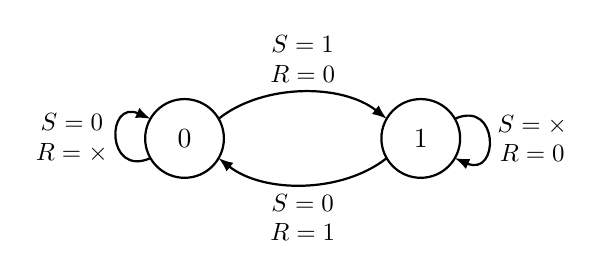
\begin{tikzpicture}
        \tikzset{style={align=center}};
        \draw[thick] (0,0) circle[radius=0.5] node {0};
        \draw[thick,-latex] ([shift={(30:0.5)}]0,0) .. controls (1,0.7) and (2,0.7) .. node[above,scale=0.9] {$S=1$\\$R=0$} ([shift={(150:0.5)}]3,0);
        \draw[thick,latex-] ([shift={(-30:0.5)}]0,0) .. controls (1,-0.7) and (2,-0.7) .. node[below,scale=0.9] {$S=0$\\$R=1$} ([shift={(-150:0.5)}]3,0);
        \draw[thick,-latex] ([shift={(30:0.5)}]3,0) .. controls (4,0.5) and (4,-0.5) .. node[right,scale=0.9] {$S=\times$\\$R=0$} ([shift={(-30:0.5)}]3,0);
        \draw[thick,latex-] ([shift={(150:0.5)}]0,0) .. controls (-1,0.5) and (-1,-0.5) .. node[left,scale=0.9] {$S=0$\\$R=\times$} ([shift={(210:0.5)}]0,0);
        \draw[thick] (3,0) circle[radius=0.5] node {1};
    \end{tikzpicture}
\end{figure}

这张图表达了所有可能的输入组合和现态会导致的次态变化。比如,如果现态$Q=1,\,S=0,\,R=1$,那么次态就是$Q^*=0$。最简单的理解方式是将$Q$和$Q^*$看成两个毫无关系的数据;在某一给定时刻,两者的确没有关系,因为只有在下一时刻,$Q^*$才会成为新的$Q$。

状态转换图是从计算理论的有限状态机中借来的表达方式。其实所有的时序电路都是有限状态机——在以后的章节中会详细探讨这一点。

\subsection*{2、真值表(特性表)和卡诺图}

所有电路的表达方式都需要在“直观”和“高效”之间做出取舍。状态转换图非常直观,但它信息密度太低,不方便后续处理。在逻辑电路中,将文字需求做初步抽象的是真值表;对于存储电路,也可以用真值表。

在状态转换图上,只要确定了输入和现态,就可以确定唯一的次态。因此,不难列出一张真值表(无效输出被作为了无关项):

\begin{figure}
    \begin{tabular}{|c|c|c|c|}\hline\rowcolor{lightgray}
        $S$&$R$&$Q$&$Q^*$\\\hline
        0&0&0&0\\\hline
        0&0&1&1\\\hline
        0&1&0&0\\\hline
        0&1&1&0\\\hline
        1&0&0&1\\\hline
        1&0&1&1\\\hline
        1&1&0&$\times$\\\hline
        1&1&1&$\times$\\\hline
    \end{tabular}
\end{figure}

和真值表等价的另一种表示方法是曾经简短介绍过的卡诺图。此处我们也可以将真值表转化为卡诺图:

\begin{figure}
    \begin{tabular}{rc|c|c|c|}
        \multirow{2}{*}{\backslashbox{$Q$}{$SR$}}&\multicolumn{1}{r}{}&\multicolumn{1}{r}{}&\multicolumn{1}{r}{}&\multicolumn{1}{r}{}\\
        &\multicolumn{1}{r}{\makebox[2em]{00}}&\multicolumn{1}{r}{\makebox[2em]{01}}&\multicolumn{1}{r}{\makebox[2em]{11}}
        &\multicolumn{1}{r}{\makebox[2em]{10}}\\\cline{2-5} 
        \multicolumn{1}{r|}{0}&0&0&$\times$&1\\\cline{2-5} 
        \multicolumn{1}{r|}{1}&1&0&$\times$&1\\\cline{2-5}
    \end{tabular}
\end{figure}

\subsection*{3、特性方程}
最后一步抽象是将真值表或卡诺图表示为方程,就好像我们之前所做的那样,甚至方法也毫无改变。因此,我们可以得出RS锁存器的函数表达:

\[Q^*=S+R'Q\]

\section*{三、RS锁存器的应用与局限}
RS锁存器最重要的用处,是将瞬时的脉冲稳定为连续的高/低电平信号。比如一个按钮,按下时输出高电平,松开便只能输出低电平,如果将其接入带一个灯泡的电路中,那只有按下按钮时灯泡才亮。但运用了锁存器后,不管按下的时间多么短暂,只要按过一次,灯泡就会保持点亮的状态。实际运用中,会用它来做开关消抖——开关拨动的一瞬间,由于簧片颤动,会输出一些不规则的高低电平信号,此时锁存器便可以将其稳定成一个从低到高的变化。

\begin{figure}
    \begin{circuitikz}[scale=0.7, transform shape]
        \ctikzset{multipoles/dipchip/width=1}
        \ctikzset{chips/scale=1.5}
        \draw (0,0) node[dipchip, num pins=6, hide numbers, no topmark,
        external pins width=0] (SR) {};
        \draw (SR.bpin 1) node[left,notcirc] {} node[right,scale={1/0.7}] {$S$} -- ++(-2,0) node (a) {};
        \draw (SR.bpin 3) node[left,notcirc] {} node[right,scale={1/0.7}] {$R$} -- ++(-2,0) node (b) {};
        \draw (SR.bpin 6) -- ++(0.8,0) node[right,scale={1/0.7}] {$Q$};
        \draw (SR.bpin 4) node[right,notcirc] {} -- ++(0.8,0) node[right,scale={1/0.7}] {$Q'$};
        \draw (a)++(0.5,0) to[R,*-] ++(0,1.5) to[short] ++(1,0) to[R] ++(0,-1.5) to[short,-*] ([xshift=1.5cm]b);
        \draw (-3.7,0) node[spdt] (Sw) {};
        \draw (Sw.in) -| ++(-0.5,-0.5) node[rground] {};
        \draw (a)+(0,0) -| (Sw.out 1);
        \draw (b)+(0,0) -| (Sw.out 2);
        \draw (a)++(1,1.5) to[short,*-] ++(0,1) node[above,scale={1/0.7}] {$V_{CC}$};
    \end{circuitikz}
\end{figure}

我们说过,锁存器的意义在于存储数据;但是,普通RS锁存器很少用作存储电路,因为它有如下局限:

\begin{itemize}
    \item S端口和R端口不能同时有效,但实际应用中不能保证这种情况不出现,此时可能会出错;
    \item 在计算机中,有许多内存单元协同组成一个寄存器,存储同一个数据。但每一位数据可能是先后到来的(比如加法器,计算出最高一位会花费比低位更多的时间),如果内存单元被写入的时间无法统一,就会造成混乱。RS锁存器并没有提供控制写入的端口——只要输入变化,状态就会改变。
\end{itemize}

对于以上问题,将会在下一章中做出改进。

封面来源:Minecraft 101
\end{document}